\subsection{Diseño del Amplificador de Audio}
\bigskip


\subsubsection{Primer Análisis}
 
El planteo comenzó focalizandose en un circuito mucho mas sencillo para el análisis. Por ende nos planteamos comprender el funcionamiento de un amplificador elemental con salida clase B como el de la Figura~\ref{idea_basica}.



\begin{figure}[H]
\centering
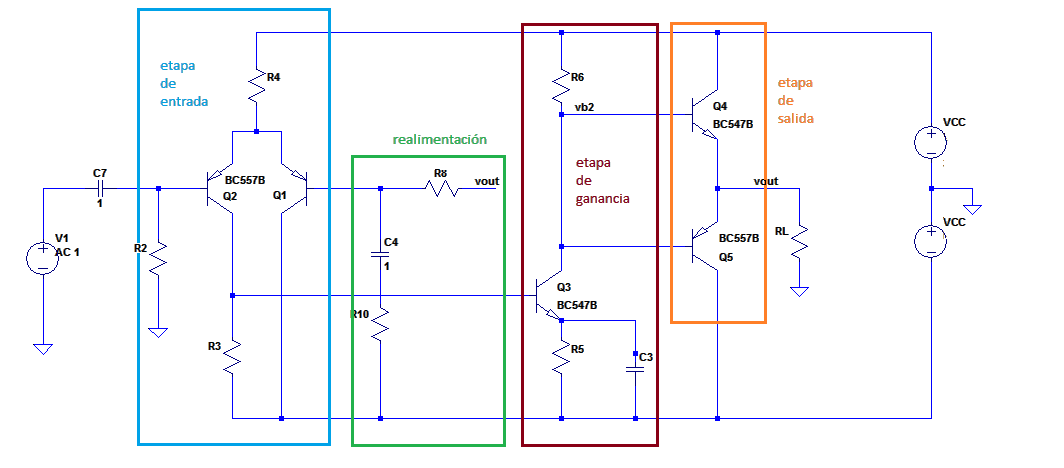
\includegraphics[width=0.8\textwidth]{img/idea_basica.png}
\caption{Amplificador simplificado.}
\label{idea_basica} 
\end{figure}

El primer desafío constó en plantear una correcta polarización. Al encontrarse el circuito realimentado negativamente es esperable que la tensión de continua en el nodo de salida $V_{out}$ sea muy cercana a cero. Este resultado puede comprenderse analizando el par diferencial y el efecto de la realimentación. Cuando el transistor Q2 se encuentre polarizado su tensión de base sea muy pequeña dado que circula una corriente baja. Por lo tanto, si la tensión $V_{out}$ no fuese un valor cercano a cero ya sea un valor negativo o positivo, produciría una tensión sobre el terminal de la base de Q1 distinto del correspondiente a Q2. Esto produciría que la corriente de Q2 se incremente o baje con respecto a la de Q1 y la salida también se vea afectada. Planteando que  $V_{out}$ aumentara:
$$
V_{out} \nearrow  ~ \Rightarrow V_{EB1} \searrow ~\Rightarrow I_{C1} \searrow ~\Rightarrow I_{C2} \nearrow ~\Rightarrow V_{B3} \nearrow ~\Rightarrow I_{C3} \nearrow \Rightarrow V_{B4} \searrow ~\Rightarrow V_{out} \searrow
$$

Siguiendo con este razonamiento si asumimos que $V_{out}$ es cercano a 0 volts. Entonces analizando el circuito llegamos a las siguientes ecuaciones:

\[
\frac{V_{CC}}{R6} = \frac{(V_{E3} - (-V_{cc})}{R5}
\]

$$
V_{E3} = V_B{3} - 0.7V
$$

Donde:
\begin{description}


\item $V_{B3} = (IC1 \times R_3 - V_{CC}) $
\item $I_{C1}=\frac{(V_{CC}-0.7V)}{2R_4}$
\item $V_{E3}= (V_{CC}-0.7) \frac{R3}{2R4} - V_{CC} - 0.7V$
\item $V_{CC} R5/R6 = \left[  (V_{CC}-0.7V) \times \frac{R_3}{2R_4} - 0.7V\right] $
\end{description}

Aproximando obtuvimos la siguiente relación:

$$ V_{CC} \times \frac{R_5}{R_6} + 0.7 =V_{CC} \times \frac{R_3}{2R_4} $$

Notando que el termino $\frac{R_5}{R_6}$ debía ser menor que la unidad debido a que $R_5$ es una resistencia de realimentación para la estabilidad de la polarización y $R_6$ es la que define la ganancia de esa etapa, y suele ser bastante alta para tener una alta ganancia de lazo abierto. 
Al tener una alta ganancia a lazo abierto la ganancia de lazo cerrado queda completamente definida por el realimentador. Observando el circuito:

$$ V_{out}= V_{in} \times \left(  1+\frac{R_8}{R_{10}} \right) ~ \Rightarrow ~ A_V= \left( 1+\frac{R_8}{R_{10}}\right) $$


Utilizando la sensibilidad requerida en las especificaciones,se estipula que al tener 1V rms en la entrada debemos tener máxima potencia de la señal de salida, asignamos a $R_8 = 22\kohm$ y a $R_{10} = 1\kohm$. De esta manera se obtiene una ganancia de 23 veces con una potencia máxima de 66 Wrms sobre una carga de $8 \ohm$ cumpliendo con los requisitos. Asignando una tensión de alimentación de $V_{cc}=35V$, simulamos el circuito:

\begin{center}
\parbox{0.5\textwidth}{
--- Operating Point ---
\begin{tabbing}
\hspace{3cm}\=\hspace{4cm}\=\hspace{5cm}\=\kill
I(Rl): \>	 -0.000492201 \>	 device$\_$current \\ 
Ie(Q1):	\> 0.000392712	\> device$\_$current \\ 
Ie(Q2):	\> 0.00116932	\> device$\_$current \\ 
I(R8):	\> -4.57521e-007\>	 device$\_$current \\ 
I(R6):	\> 0.000730688	\> device$\_$current \\ 
I(R5):	\> 0.000731219	\> device$\_$current \\ 
I(R3):	\> -0.00116632	\> device$\_$current \\ 
I(R2):	\> -1.36041e-006\>	 device$\_$current \\ 
I(R4):	\> 0.00156204	\> device$\_$current \\ 
\end{tabbing}
}
\end{center}

\begin{figure}[H]
\centering
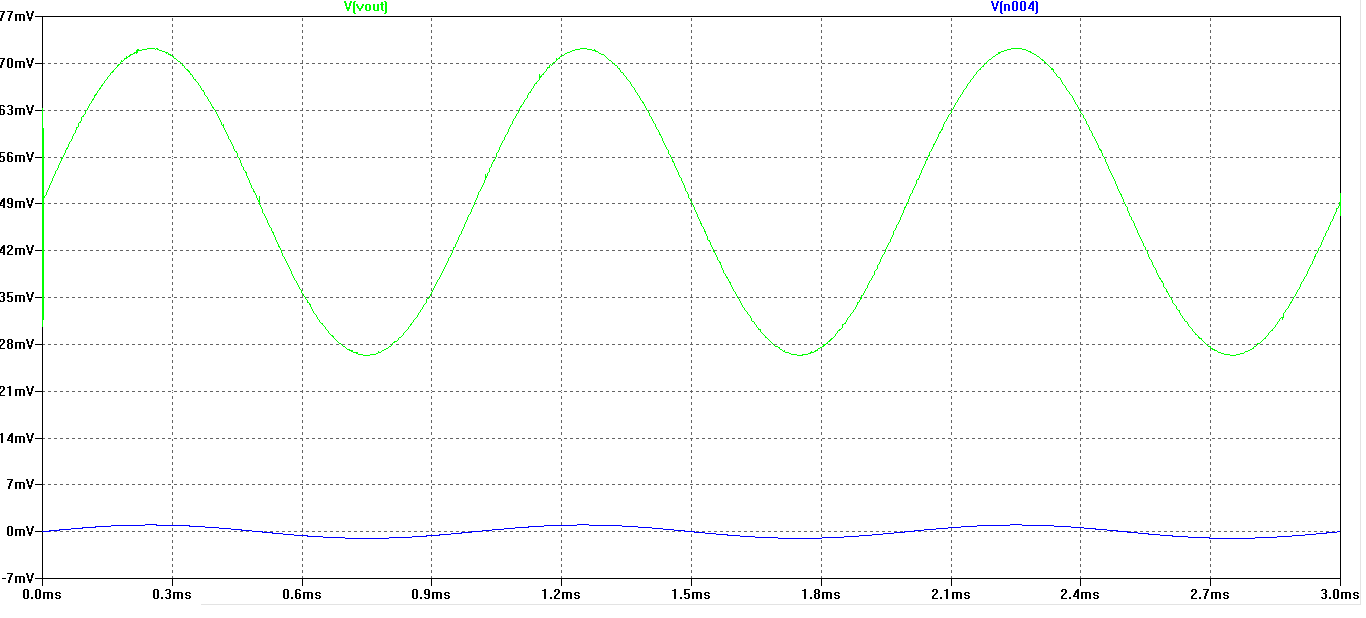
\includegraphics[width=\textwidth]{img/ganancia_1er_cir.png}
\caption{Respuesta temporal del $1^{er}$ prototipo.}
\end{figure}

\begin{figure}[H]
\centering
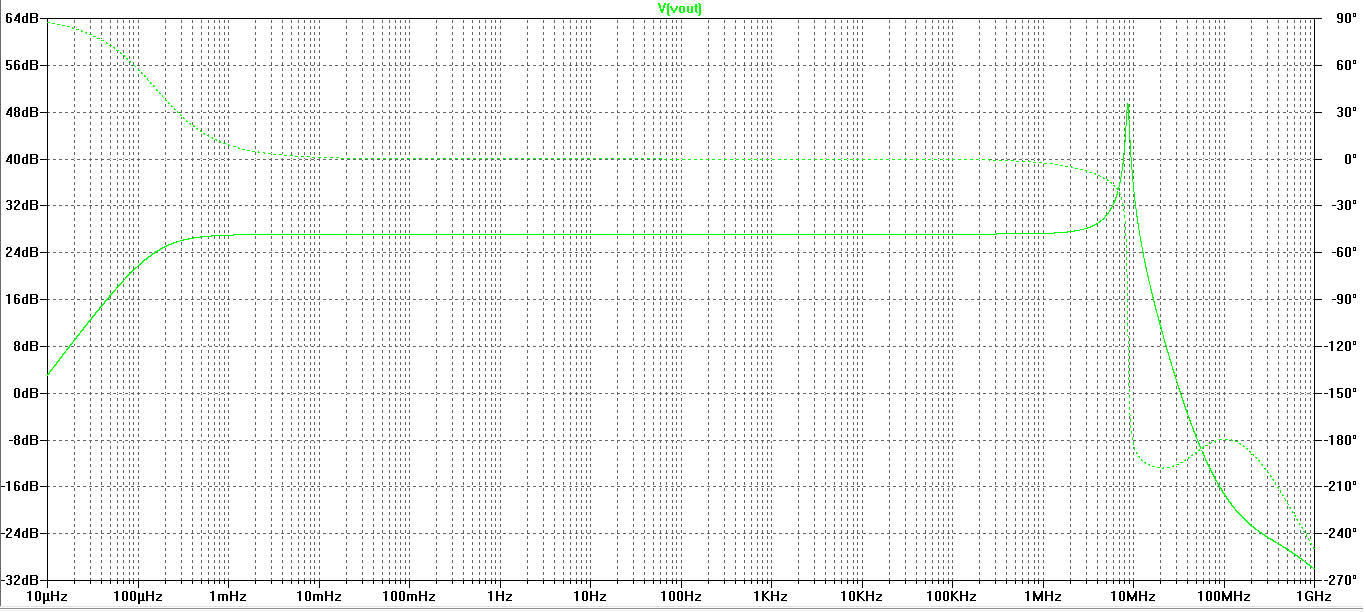
\includegraphics[width=\textwidth]{img/cir_basico_oscilante.png}
\caption{Respuesta en frecuencia del $1^{er}$ prototipo.}
\end{figure}

Los valores asignados fueron elegidos con el criterio de lograr una corriente de alrededor de 1mA para la etapa de entrada y de una relación entre $\frac{R5}{R6}$  de 0.001 veces. Obteniendo el resultado de que el circuito amplifica 22.85 veces y posee una alta inestabilidad.
Notar que el circuito simulado posee una resistencia de carga de 100 $\ohm$. Realizando una simulación habiendo compensado el circuito para que no se produzcan oscilaciones se obtuvo:

\begin{figure}[H]
\centering
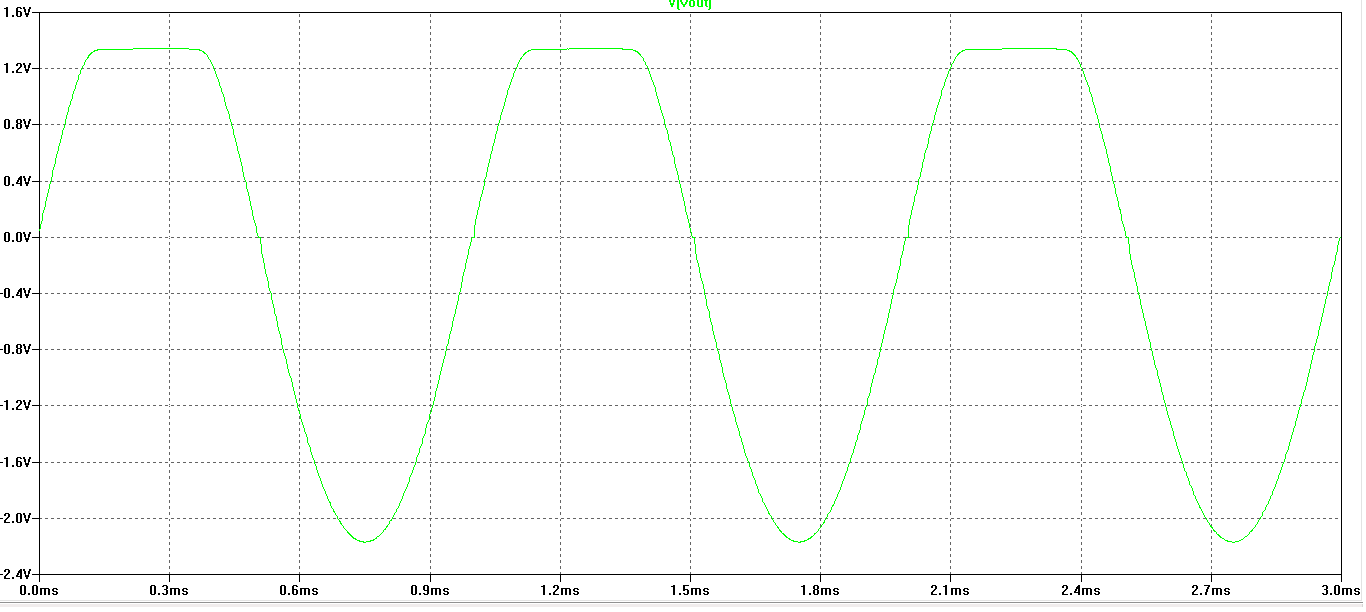
\includegraphics[width=\textwidth]{img/cir_basico_compensado.png}
\caption{Respuesta temporal luego de compensar.}
\end{figure}

Como puede observarse otro cambio que deberíamos lograr era bajar la resistencia de salida del circuito para que etapa de salida pudiese entregar mayor potencia sin llegar al recorte. Por ende aplicando una cantidad significativa de cambios pasamos a analizar el siguiente circuito:

\begin{figure}[H]
\centering
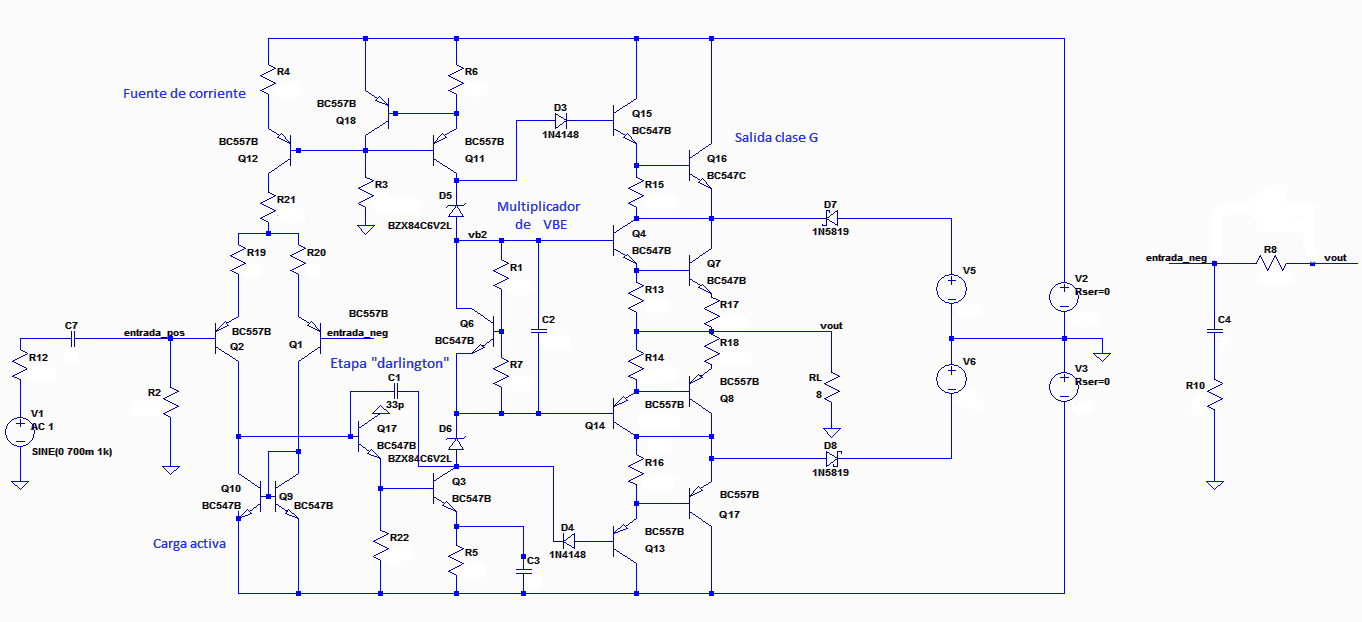
\includegraphics[width=\textwidth]{img/circuito_beta_mejorado.png}
\caption{Amplificador básico con algunas mejoras.}
\end{figure}

La primer diferencia que podemos apreciar es el reemplazo de la resistencia $R_4$ del circuito anterior por una fuente de corriente. Este cambio logra que la corriente de polarización del par diferencial sea mas estable frente a variaciones tanto por parte de la fuente de alimentación como así también por la temperatura de operación. Esta corriente es vital para definir las propiedades de pequeña señal y las distorsiones que puedan ocurrir en la primer etapa.Ademas aumenta su relación de rechazo en modo común.
Para calcular dicha corriente recorreremos la malla de control de dicha fuente aplicando la ley de Kirchhoff obtenemos que:
$$
V_{2} - V_{R4} - V_{BE Q12} + V_{BE Q11} + V_{R6} - V_{2} = 0
$$
Asumiendo que los dos transistores son exactamente iguales podemos asumir que sus $V_{BE}$ también lo serán. Por ende:
$$
- I_{C Q12} * R_{4} + I_{C Q11} * R_{6} = 0
$$
Llegando a la siguiente relación:
$$
I_{C Q12} = I_{C Q11} \times \frac{R_6}{R_4}
$$
\\
Por ende las corrientes $I_{C Q12}$ e $I_{C Q11}$  quedan determinadas por la relación entre $R_6$ y $R_4$. Para calcular la corriente $ I_{C Q11}$ realizamos la suposición de que el la tensión $V_{BE Q18}= 0,7V$ y en consecuencia $I_{C Q11}= {V_{BE Q18}}/{R_6}$. Los valores de resistencias normalizados adoptados logran que la corriente del par diferencial se mantenga alrededor de 1 mA. Este valor lo establecimos como norma, ya que valores mayores incorporarían más ruido a la primera etapa, y valores menores disminuirían la ganancia.

La segunda gran diferencia es la aplicación de una carga activa en reemplazo de resistores en el par diferencial lo cual nos introduce un aumento en la amplificación sumado a que se logra un lazo de realimentación que estabiliza la polarización, es decir, tiende a igualar las corrientes por ambas ramas del amplificador diferencial, disminuyendo los efectos de los desapareamientos e impidiendo la aparición de distorsión por $2^{da}$ armónica.

La tercer diferencia radica en la modificación de la etapa de ganancia por una etapa darlington para aumentar aun más la ganancia de lazo abierto. Además en esta etapa se ha colocado un capacitor, $C_1$, entre la base y el colector, de lo que sería $Q_3$ del circuito anterior, que produce un polo dominante para altas frecuencias. Este tipo de compensación se basa en el hecho de que la ganancia de la etapa es lo suficientemente grande como para que la capacitancia reflejada por efecto Miller también lo sea. La ventaja es que con capacidades pequeñas se logra estabilizar el sistema y estas suelen venir incluidas en el circuito integrado. La realimentacion local que linealiza la etapa se ve incrementada tal que a fines prácticos elimina la distorsion por alinealidad totalmente. La carga del colector del VAS, $Q_9$, forma una fuente de corriente, y se agrega el capacitor $C_3$ para que no haya realimentación en señal, aumentando así la ganancia.

La cuarta diferencia es la utilización de un circuito adicional entre las bases de $Q_5$ y $Q_4$. Posee dos funciones elementales: la primera es establecer una corriente de polarización en los transistores de salida que produce una notable disminución de la distorsión por cruce por cero. Para entender este efecto analizamos el primer circuito planteado, como observamos cuando un transistor de la etapa de salida clase B se encuentre el conducción el otro se encuentra en corte. Al disminuir la tensión de la salida del emisor común ($2^{da}$ etapa) a niveles cercanos al cero, ninguno de los transistores se encuentra en la región activa y en ese instante se produce una deformación de la señal como se observa en la Figura~\ref{falta_Vbe}. Claramente este tipo de distorsión será mas apreciable a señales de baja amplitud donde los efectos son mas apreciables. Para modificar este comportamiento se agregaría una "fuente" de tensión entre las bases de la etapa de salida clase B. Esta fuente polariza ambos transistores y produce por los mismos una corriente constante dependiendo exponencialmente de su valor. Esta "fuente" es reemplazada por el multiplicador donde como se ha analizado en clase, si el mismo es alimentado con una fuente de corriente constante vale afirmar que:

$$
V_{CE Q6} = (\frac{R_1}{R_7} + 1 ) \times V_{BE Q6}
$$

\begin{figure}[H]
\centering
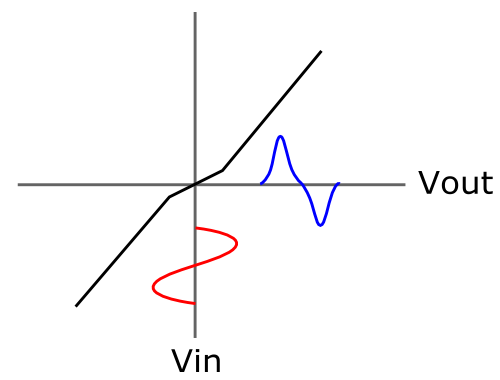
\includegraphics[width=0.5\textwidth]{img/falta_Vbe.png}
\caption{Deformación por falta de Multiplicador $V_be$}
\label{falta_Vbe}
\end{figure}

Ahora bien la segunda función elemental se observa en esta ecuación. El transistor $Q_6$ del multiplicador se acoplará termicamente con la etapa de salida de forma tal que si estos transisitores se embalan termicamente, es decir, un aumento de la temperatura produce un aumento de corriente que vuelve a producir un aumento de temperatura. Pero si el transistor $Q_6$ esta acoplado terminamente con la etapa de salida, al aumentar la temperatura pruducira una disminución en el valor de la tensión $V_{BE}$ (-2mV/$^o$C), disminuyendo la tensión $V_{CE Q6}$, bajando la corriente de los transistores y produciendo un lazo de realimentación negativa. El capacitor $C_2$ se agrega para corregir la impedancia inductiva que muestra este multiplicador al resto del circuito.

La quinta gran diferencia es la utilización de otro tipo de etapa de salida, la llamada clase G. Esto se relaciona al hecho de que quiere utilizarse para la reproducción de música, la cual, la mayor parte del tiempo se encuentra en niveles bajos y solo tiene picos temporales. Este hecho hace que sea eficiente el uso de una salida clase G.

En esta etapa los transistores están en configuración seguidor por emisor, ya que es sabida de ser menos propensa a oscilaciones parásitas o locales. $R_{15}$ y $R_{14}$  son los clásicos resistores de emisor para los drivers de bajas. Los drivers $Q_{12}$ y $Q_{15}$ tienen sus propios resistores de emisor $R_{13}$ y $R_{16}$, que cumplen su rol de establecer una razonable corriente en los drivers cuando se prenden a modo de incrementar su transconductancia y ademas acelerar el apagado de los dispositivos de altas al proveer una salida para los portadores de las bases de los mencionados dispositivos. Los colectores de los drivers están conectados a los rieles de altas para minimizar los saltos de ganancia causados por el cambio abrupto en la tension de colector cuando se produce la conmutación.

Cuando una tension positiva excede el riel de bajas($D_6$ y $D_5$ son los responsables de definir cuando se utilizara el riel de bajas o altas), $D_3$ pasa a conducción,$Q_{15}$ y $Q_{16}$ se prenden mientras que $D_7$ se apaga y , por lo tanto, la corriente es suministrada  el riel de altas, con la caída de tension y consumo de potencia debidos a $Q_{15}$ y $Q_{16}$. Los picos de tensiones negativas tienen un desarrollo análogo.
La conmutación en la clase G trae acarreado un problema de alinealidad en los diodos de conmutación. Estos diodos en general deben conducir grandes cantidades de corriente antes de conmutar, y una consiguiente acumulación de cargas. Al conmutar las cargas acumuladan mantienen la corriente durante un corto tiempo mientras son barridas de la juntura. Esta corriente es suministrada por el transistor de altas. Cuando el diodo corta completamente, este exceso de corriente que conducía el transistor de altas pasa directamente hasta el de bajas y a la resistencia de degeneración. Este problema se puede eliminar con un diodo de alta recombinación, como ser el diodo Schottky de potencia, que son mas rápidos y acumulan menos carga.

Mientras la señal se mantenga en baja potencia, un amplificador de baja potencia lo hará mas eficiente. La mayor parte del tiempo son los rieles de baja tension los que proveen la potencia de salida, habiendo baja caída de tension entre riel y salida y consecuentemente, menor disipación. Pero, cuando aparecen picos de alta tension, se activan los rieles de alta tension, causando mayor gasto de energía durante esos cortos periodos de tiempo.

Modificando levemente al circuito anterior para mejorar algunas propiedades y agregando bloques para obtener nuevas características, resultara el esquema de la Figura~\ref{im:circuito}. Se detallarán estas modificaciones y se calcularán los valores de todos los elementos utilizados para su implementación.

\begin{figure}[H]
\centering
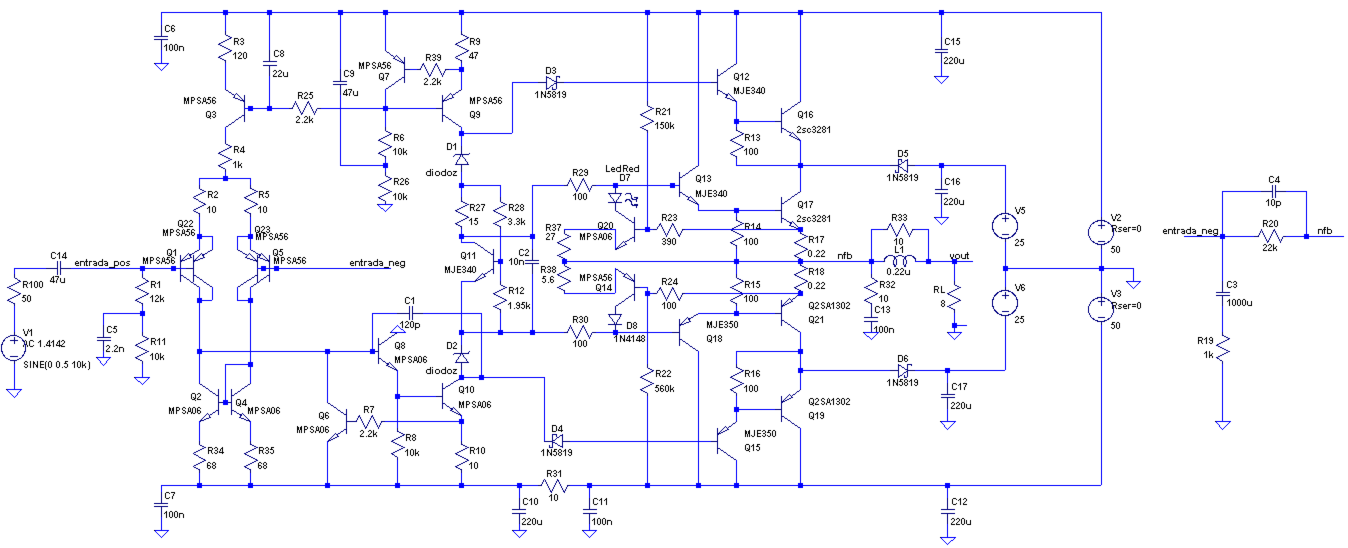
\includegraphics[width=\textwidth]{img/circuito.png}
\caption{Amplificador que se implementará.}
\label{im:circuito} 
\end{figure}


Como se puede observar, tanto $Q_{14}$ y $Q_{20}$ $Q_{6}$como (como sus resistencias y diodos relacionados) componen circuitos de protección contra cortocircuitos. El funcionamiento básico es que usa los resistores de la salida para sensar la corriente que pasa por ellos. Cuando la corriente excede el valor máximo permitido, el cual se elige para una sobrecarga determinada (esto incluye el caso extremo de cortocircuito), la tensión que cae en esta resistencia enciende en transistor, el cual comienza a drenar corriente de la entrada de la etapa de salida, a fin de limitar la corriente de salida.
Un problema que se podría tener es el de tener un corto interno pero no notarlo, en cuyo caso las protecciones estarían constantemente en funcionamiento. Entonces, para notarlo, se reemplazo un diodo de las protecciones por un LED, a fin de que cuando las protecciones esten funcionando, el LED se polarice y su señal luminosa nos informe del problema.

La entrada diferencial también fue modificada, $C_5$ ayuda a fijar la impedancia para señal, sin afectar la "vista" en polarización por la entrada del mismo. Esto ultimo es importante ya que para minimizar desapareamientos es recomendable que ambas entradas del par tengan la misma resistencia en polarización. Otra modificación es la utilización de dos transistores en paralelo a la entrada, esto produce dos beneficios. El primero es debido a que los $\beta$ equivalentes de cada par de transistores son más similares entre si que dos $\beta$ individuales debido a la dispersión de los mismos,disminuyendo así el desapareamiento. El segundo beneficio se debe a que la corriente de polarización que fluye por cada transistor es la mitad que antes, disminuyendo así el ruido Shot generado por estos transistores.

Otra pequeña modificación es el agregado de la resistencia $R_{27}$ al multiplicador $V_{BE}$, para independizarlo de la corriente que circula por el mismo.

Un componente fundamental agregado en este último circuito es el capacitor $C_4$ en la realimentación, esta puede usarse para compensar por adelanto de fase y así no depender exclusivamente de $C_1$ para definir la respuesta en altas frecuencias.

Para alimentar todo el circuito se han utilizado el par positivo y negativo de rieles de alta tensión. Sin embargo hay un pequeño circuito RC que filtra los rieles que van a las etapa VAS y de entrada. Esto las provee de una fuente de tensión mucho mas limpia que la porción de alta corriente de ese mismo riel, que alimenta a la etapa de salida. Esta porción de riel siempre tiene mucho ripple y ruido que contaminaría las etapas mas sensibles de no ser filtrada.

A la salida se agrego un bloque que mejora la relación entre el amplificador y su carga. $C_{13}$ y $R_{32}$ conforman la red Zobel encargada de prevenir inestabilidades en altas frecuencias debido a cargas demasiado inductivas. La red conformada por $L_{1}$ y $R_{33}$ aíslan al amplificador de carga capacitiva, aplanando la respuesta en frecuencia.

Con la topologia actual se procederá a seleccionar los valores de los componentes utilizados. 
\medskip


%La resistencia de entrada desacoplada por el capacitor C5 provee una resistencia de entrada de $10K\Omega$ para la señal y en continua se ven $22K\Omega$, equiparando con la realimentacion. De esta forma, se equilibra el offset producido por las corrientes de base del par diferencial, minimizando la tensión diferencial de offset.

%El principal inconveniente al compensar el circuito por polo dominantes es que al agregar un capacitor, este modifica el ancho de banda de potencia. Esto se debe al tiempo que le toma a la etapa anterior cargar el capacitor. Debido a esto la elección del valor de este capacitor debe tener en cuenta ambos efectos y buscar una relación de compromiso entre ambos.

%\subsubsection*{Slew Rate}
%
%El capacitor de compensación $C_1$ conectado alrededor del par Darlington hace que esta etapa actúe como un integrador, y la corriente que carga el punto de compensación es justamente $I_x$. 
%Se puede observar que la corriente máxima disponible para cargar C1 es 2$I_1$, donde $I_1$ es la corriente en reposo por cada dispositivo en la etapa de entrada. Es decir, a grandes valores de Vi las corrientes del par diferencial se desequilibran, $I_1$ crece hasta su valor máximo 2$I_1$ y la corriente por la otra rama del par se anula, por ende es fácil ver que por la carga activa deja de circular corriente y toda la corriente de la primer rama del par se transforma en $I_x$.
%El circuito por lo tanto opera en forma no lineal. Si la etapa de entrada actuara de forma lineal produciría una corriente $I_x$ muy grande y el slew rate no produciría ninguna limitación.
%
%\[
%	V_o= \dfrac{1}{C1} \int 2I_1\,\mathrm{d}t    
%\]
%
%$$
%	SR=\dfrac{dVo}{dt}=\dfrac{2I_1}{C1}
%$$
%
%Por lo tanto, realizando el calculo para nuestro circuito, siendo $I_1$ =2.2mA y C1=120pF. Obtenemos:
%$$ SR=36\dfrac{V}{\usec} $$


\bigskip